\section{Related Work}

\subsection{IVR \& Asynchronous Audio}

By allowing users to interact with digital systems through standard phone calls using their phone's keypad (and sometimes even their voice \cite{khullar2021}), Interactive Voice Response (IVR) systems have been shown to be an effective tool for information retrieval and exchange: especially in low-resource contexts where users have limited internet access \cite{eitzinger2019} and low literacy inhibits the usability of text-based interfaces \cite{sharma2009}. IVR and asynchronous audio has proven to be a versatile medium, with previous projects utilising it in a wide variety of contexts and use cases, including: performing voice-based surveys \cite{khullar2021_surveys}; supporting users in accessing information on-demand \cite{Riaz2017} or using multi-modal voice browser \cite{mahelaqua2013}; connecting offline workers to online marketplaces \cite{Richardson2022}; connecting families in different time zones using multiple devices, where users can have a feeling of sharing their stories, activities, and time \cite{heshmat2020}; enabling citizen journalism \cite{Ejaz2018}; creating `voice forums', where users can create and respond to audio messages through phone calls \cite{Patel2010, Vashistha2015}; social networking of farmers \cite{Indrani2015}; and interacting with automated conversational agents (`chatbots') to access information \cite{Jain2018, Yadav2019}. These systems offer greater accessibility to users from communities with oral traditions \cite{Ndwe2012}, and can be designed to support cost-free, on-demand access to end-users \cite{Richardson2022, zhang1998}. Additionally, prior studies have highlighted the value of being able to access recordings for later reference on-demand \cite{Talhouk2017}, with the ability to repeatedly access the same information being useful for low-literate users who cannot write information down \cite{Jain2018}. 

Despite the versatility and scalability afforded by this infrastructure, however, automated IVR systems aren't always able to fulfill users' highly specific and contextual queries: traditional IVR menu structures are limited in scope, requiring designers to choose what information and interactions should be prioritised \cite{Richardson2022}. Chatbots have been shown to be able to respond accurately to highly specific queries \cite{Jain2018}, but such systems are dependant on currently unreliable speech-to-text systems and access to extensive databanks of previous responses by human experts. Furthermore, for users unfamiliar with the limitations of chatbots, interacting with them can clash with expectations of interacting with a human over the phone \cite{Jain2018}: resulting in conversational queries which humans could interpret correctly, but automated systems struggle with \cite{Yadav2019}. Meanwhile, voice forums offer human replies, but the ability for anyone to respond to queries can lead to misinformation \cite{Patel2010}, as well as harassment, threats, and systemic marginalisation towards women and minorities \cite{Vashistha2019}.

\subsection{Radio \& Synchronous Audio Platforms}
\label{section:talkshow}

Synchronous voice formats, such as radio, can address these issues through direct moderation of a synchronous activity by a host. Often run by volunteers, community radio stations broadcast live audio content to local communities: offering a method for civic engagement, deliberation and knowledge sharing \cite{Cibin2019, Maye2020}. Projects such as RootIO have drastically lowered the costs of radio infrastructure and encourage community-led participatory programming \cite{Csik2016}, particularly when combined with technologies for generating audio content, such as text-to-speech \cite{Scott2020}. Unfortunately, while many radio programmes offer the ability for audiences to call into a show to ask questions, by default radio is an inherently passive medium in terms of audience interaction. Furthermore, broadcast radio often requires the navigation of local policy and broadcast content standards: erecting legal, logistical and psychological barriers due to formal license applications and requirements \cite{Maye2020, Bidwell2021}.

In recent years, researchers such as Kazakos et al. \cite{Kazakos2016} have begun sidestepping these barriers by providing access to `radio' programming through phone-based platforms: hosting live shows through synchronous telephony, with listeners able to dial in with their phones to listen and ask questions to a host controlling the show from a smartphone or web application. These platforms use free, `off the shelf' software such as FreeSWITCH\footnote{\url{https://signalwire.com/freeswitch}} to programmatically manipulate phone calls. 

In these platforms \cite{Kazakos2016, Talhouk2017, Yadav2017}, participants join an engagement by either receiving a phone call or initiating a `callback' (where the system hangs up on incoming calls and immediately calls them back, so that participants aren't charged). Participants spend the majority of the engagement muted, passively listening to one or more unmuted users: a `host' user and, if present, guests (typically experts in their field, e.g. healthcare providers \cite{Talhouk2017}). These discussions are typically unscripted. The engagements often also have a question and answer (Q\&A) segment, where members of the audience can request to be unmuted by pressing a button on their phone. The host can see these requests through a visual interface, and choose who to unmute and when to re-mute them. The audience member's question would then be discussed by the host and/or guests before moving onto the next question. Some platforms also support the recording and playback of audio during the call \cite{Talhouk2017, Yadav2017}.

Yadav et al. note the potential for such platforms to go beyond the `radio' model by additionally supporting asynchronous pre- and post- show interactions, where the audience could dial into the system to submit questions or relisten to prior content on demand \cite{Yadav2017}. As Kazakos et al. (and follow-up investigations by researchers using similar systems \cite{Talhouk2017, Yadav2017}) demonstrate, synchronous telephony allows for remote group engagements with a low barrier to entry, and offers the potential for active audience participation: bringing education, training, and individuals' specific expertise into the homes of rural and underprivileged communities, for whom such knowledge might otherwise have been inaccessible.

Despite this promise, however, these platforms still feature significant design limitations: taken as described in their publications, they are all configured exclusively around the `talk show' concept, with the call host primarily leading discussions with a domain expert and fielding questions from the (otherwise muted) listening audience. These projects have highlighted a number of challenges with this format: for example, a dependence on questions can lead to `content black holes' when they are not received \cite{Kazakos2016}; and while this can be mitigated through pre-prepared audio content \cite{Yadav2017}, an over-reliance on recorded audio and muted participants doesn't take full advantage of the dynamic possibilities of synchronous audio, nor the two-way nature of typical telephone interactions. Furthermore, there is an asymmetrical power imbalance embedded in the talk show design pattern: the call's host has a visual overview and control over the call and its participants, while others---outside of requesting to be unmuted---are relegated to being passive consumers \cite{Varghese2022}. This would make the format unsuitable in contexts which value more open, free-flowing and unbiased discussion \cite{Fiesler2019}, or those that require structured procedure to allow for equal opportunities for participation \cite{robert2020}. Due to the specialisation of these projects and their lack of separation between the concerns of engagement design and core infrastructure, in practice any context which requires an engagement archetype that significantly differs from a talk show necessarily requires the design and implementation of a new, custom-built platform.

\subsection{Ontologies, Design Vocabularies, \& Group Telephony}

Having an agreed-upon terminology to describe the components, behaviours, and characteristics of emerging or underexplored technologies can support the design, development and comparison of implementations of them. `\textit{From a purely computational standpoint, the ontology of a system lies at the heart of its ability to represent elements of the physical world}' \cite{Brubaker2011}. Formal ontologies are often produced with this use-case in mind: intended to create `\textit{a shared and common understanding of some domain that can be communicated across people and computers}' \cite{struder1998}. They can be used to create and communicate consensual conceptual models (referred to as `domain reference' ontologies), which can then be further developed to be used to support semantic interoperability within automated systems (referred to as being `operational') \cite{guizzardi2007} when written in a machine-interpretable language such as OWL (Web Ontology Language\footnote{\url{https://www.w3.org/OWL/}}). To support extensibility and reusability, ontologies are frequently organised within three tiers: \textit{foundational}, which describe fundamental concepts that can be shared and reused across many fields (e.g. `a thing'); \textit{core}, which build upon foundational axioms to provide abstract definitions more specific to a particular field (e.g. `a document is a thing'); and \textit{domain}, a definition of concepts and relations concerning a specific, specialised domain (e.g. `a forum post is a document') \cite{scherp2011}. Costa et al. note that ontologies have been used to structure and infer knowledge, support reasoning, and serve as a basis for developing systems or frameworks across many portions of the CSCW and HCI domains---such as within user interface design, ubiquitous computing, user modeling, design methods, usability, and accessibility \cite{costa2021}. 

Beyond formal ontologies, other approaches have been used within CSCW and HCI to describe and illustrate the characteristics of technologies and interactions with them. For example, Kamran et al. proposed a social semantic tagging system, Collaborative Ontology Development, that dynamically updates user and web content identities based on the evolving collective opinion of relevant user communities in the `Entrepreneurship' domain, thereby fostering collaboration, networking, and knowledge sharing in the field of entrepreneurship \cite{Kamran2016}. Kharrufa et al. contributed a conceptual model which allowed for the visual communication of different approaches to user identification on multi-touch devices: aiming to support non-technical practitioners to compare the common parameters that characterize them, independent of their specific use-cases \cite{Kharrufa2017}. Similarly, Chuang et al. produced a `design vocabulary' to describe user-computer communication within IoT systems, supporting the comparison and design of different forms of interaction \cite{Chuang2018}. In comparison to the aforementioned machine-interpretable ontologies which focus on describing existing implementation, these examples instead place greater focus on future design: communicating a system's requirements, strengths, limitations, or possibility space through the use of visuals and hypothesised future technologies. 

\begin{figure}[h]
  \centering
  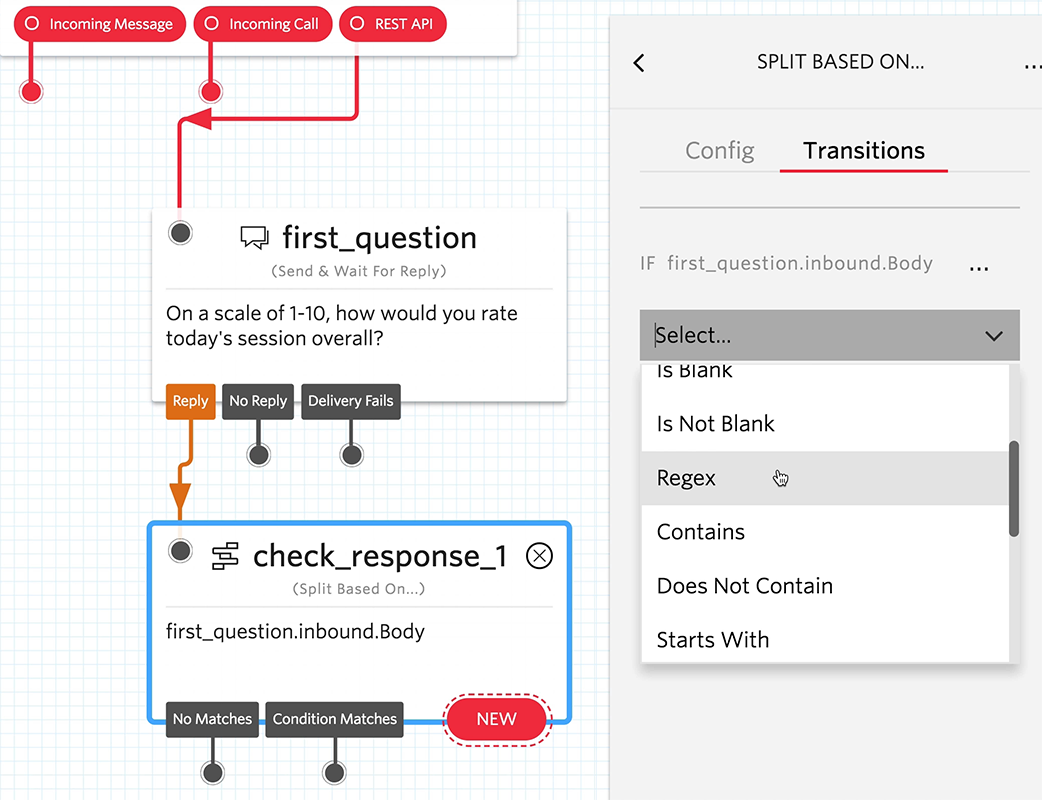
\includegraphics[width=0.6\linewidth]{images/twilio.png}
  \caption{Twilio's Studio interface, which allows for producing IVR logic through a visual programming interface.}
  \Description{A screenshot of Twilio's Studio interface. It shows a GUI in a flow chart style format, with nodes connected by arrows. The first node in the chain is "REST API", and connects with an arrow to a card titled "first question". This card contains the text "on a scale of 1-10, how would you rate today's session overall?". The card has exit nodes titled "Reply", "No Reply", and "Delivery Fails". The "Reply" node is connected by an arrow going to a second card, titled "check_response_1", which is currently being produced by the script author.}
  \label{fig:twilio}
\end{figure}

While prior works have explored the use of ontologies to drive contextual dialogues in IVR systems \cite{ababneh2013, thirumaran2015, thirumaran2015a}, detail the technical aspects of radio transmission and operation \cite{ihmcIHMCOntology}, describe media industry production workflows \cite{movielabs2021}, and support the automatic processing and annotation of meetings \cite{niekrasz2006}, we have not identified an ontology or design vocabulary that describes the configuration and composition of synchronous group interaction archetypes, or how they can be scaffolded or facilitated remotely through telephony. Tools do exist to rapidly develop (and therefore describe) IVR platforms using visual interfaces (e.g. Twilio Studio\footnote{\url{https://www.twilio.com/serverless/studio}}), allowing users to scaffold IVR interactions without requiring significant programming experience through a visual representation of logic (Figure \ref{fig:twilio}). However, these tools largely focus on the design of asynchronous interactions (e.g. SMS surveys, IVR menus) or connecting callers to separately handled synchronous activities (e.g. a helpline), without describing or offering granular controls over synchronous group interactions. As such, there exists a need for a set of agreed upon terms and metaphors to assist designers in conceptualising, visualising, and communicating synchronous group telephony systems and interactions.